% -*- TeX:de -*-
\NeedsTeXFormat{LaTeX2e}
\documentclass[12pt,a4paper]{article}
\usepackage[german]{babel} % german text
\usepackage[DIV12]{typearea} % size of printable area
\usepackage[T1]{fontenc} % font encoding
%\usepackage[latin1]{inputenc} % most likely on Windows
\usepackage[utf8]{inputenc} % probably on Linux
\usepackage{multicol}

% PLOTTING
\usepackage{pgfplots} 
\usepackage{pgfplotstable}
\usepackage{url}
\usepackage{graphicx} % to include images
\usepackage{tikz}
\usepackage{subfigure} % for creating subfigures
\usepackage{amsmath} % a bunch of symbols
\usepackage{amssymb} % even more symbols
\usepackage{booktabs} % pretty tables

% a floating environment for circuits
\usepackage{float}
\usepackage{caption}

%\newfloat{circuit}{tbph}{circuits}
%\floatname{circuit}{Schaltplan}

% a floating environment for diagrams
%\newfloat{diagram}{tbph}{diagrams}
%\floatname{diagram}{Diagramm}

\selectlanguage{german} % use german

\begin{document}

%%%%%%% DECKBLATT %%%%%%%
\thispagestyle{empty}
			\begin{center}
			\Large{Fakultät für Physik}\\
			\end{center}
\begin{verbatim}


\end{verbatim}
							%Eintrag des Wintersemesters
			\begin{center}
			\textbf{\LARGE WS 2013/14}
			\end{center}
\begin{verbatim}


\end{verbatim}
			\begin{center}
			\textbf{\LARGE{Physikalisches Praktikum\\ für das Bachelorstudium}}
			\end{center}
\begin{verbatim}




\end{verbatim}

			\begin{center}
			\textbf{\LARGE{PROTOKOLL}}
			\end{center}
			
\begin{verbatim}





\end{verbatim}

			\begin{flushleft}
			\textbf{\Large{Experiment (Nr., Titel):}}\\
							%Experiment Nr. und Titel statt den Punkten eintragen
			\LARGE{PW1, Messen - Messfehler}	
			\end{flushleft}

\begin{verbatim}

\end{verbatim}	
							%Eintragen des Abgabedatums, oder des Erstelldatums des Protokolls
			\begin{flushleft}
			\textbf{\Large{Datum:}} \Large{17.10.2013}
			\end{flushleft}
			
\begin{verbatim}
\end{verbatim}
							%Namen der Protokollschreiber
		\begin{flushleft}
			\textbf{\Large{Namen:}} \Large{Patrick Braun, Johannes Kurz}
			\end{flushleft}

\begin{verbatim}


\end{verbatim}
							%Kurstag und Gruppennummer, zb. Fr/5
			\begin{flushleft}
			\textbf{\Large{Kurstag/Gruppe:}} \Large{DO/2}
			\end{flushleft}

\begin{verbatim}



\end{verbatim}
							%Name des Betreuers, das Praktikum betreute.
			\begin{flushleft}
			\LARGE{\textbf{Betreuer:}}	\Large{Johanna Akbarzadeh}	
			\end{flushleft}

%%%%%%% DECKBLATT ENDE %%%%%%%
\pagebreak
\setlength{\columnsep}{20pt}
\begin{multicols}{2}
\section{Einleitung}
In diesem (ersten) Praktikumsbeispiel geht es um Messen, Messfehler und -unsicherheiten.
Da Messung ein (wenn nicht "der") Bestandteil eines jeden Experimentes ist, ein Thema, das sich durch alle Bereiche, nicht nur der Physik zieht, steht diese Aufgabenstellung am Anfang des Anfängerpraktikums und ist aufgeteilt auf 3 kleinere Beispiele aus unterschiedlichen Bereichen:\\
\textbf{Längenmessung:} die Stärke eines Kupferdrahtes wurde mittels unterschieldicher Methoden gemessen\\
\textbf{Zeitmessung und Unsicherheit:} die Bestimmung der Gravitationsbeschleunigung durch die Schwingungsdauer eines Fadenpendels\\
\textbf{Spannung/Strom:} Bestimmung von Widerständen durch die Messung von Strom und Spannung in einfachen Netzwerken\\
\\
Neben dem Titel der Einheit, ist den Beispielen eine Einführung in verschiedene grundlegende Messgeräte gemeinsam, sowie erste Erfahrungen im Aufbau einfacher Experimente, gleichzeitiger erster on-the-fly-Überprüfungen der gemessenen Werte sowie Fehlerminimierung.\\
\\
Aufgrund der Struktur der Praktikums-Einheit, ist also auch dieses Protokoll in 3 Teilen gegliedert:\\
TODO 1\\
TODO 2\\
TODO 3\\

\section{Einfache mechanische Messungen}
\subsection{Bestimmung der Dicke eines Kupferdrahtes (und ein Dreieck)}
\begin{figure}[H]
	\centering
  	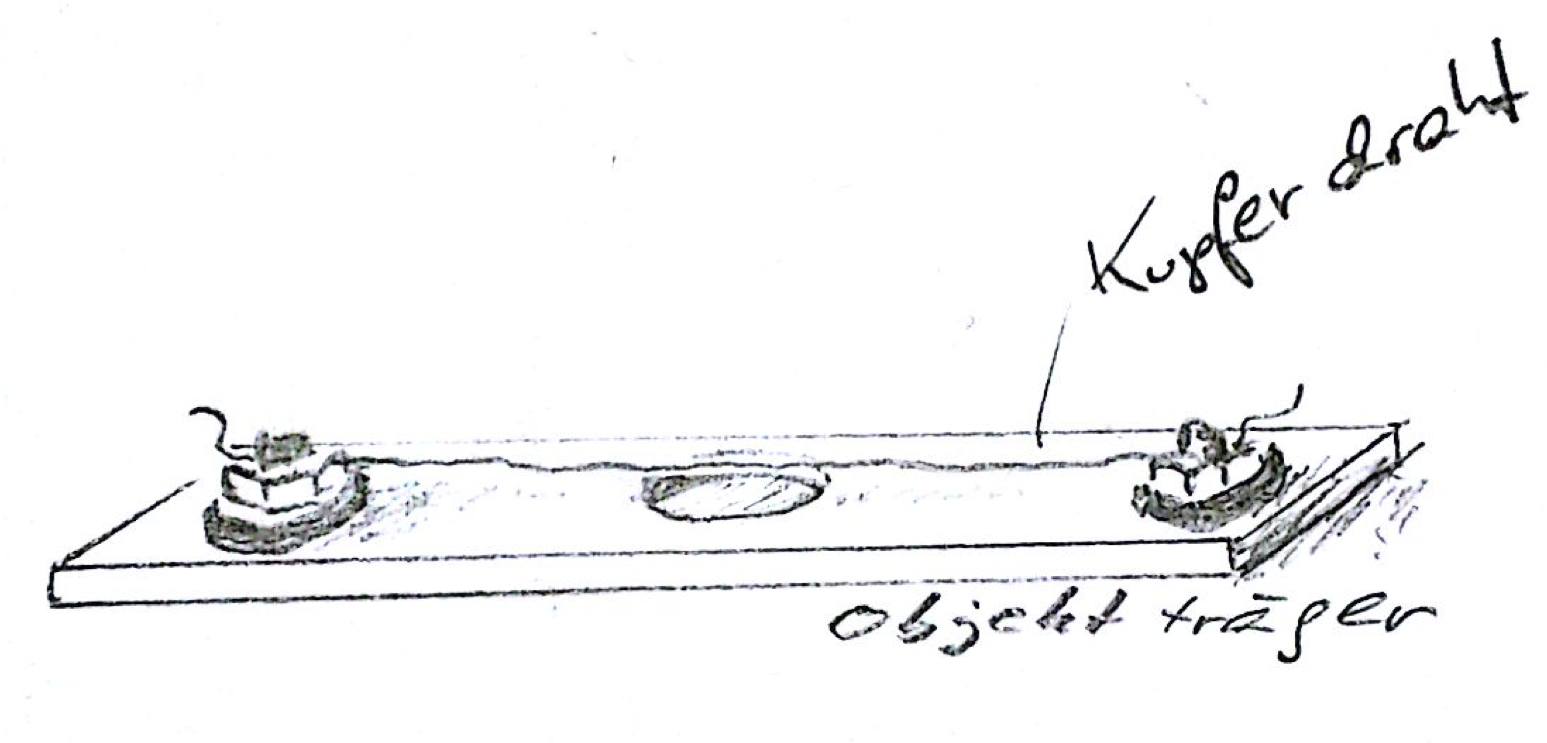
\includegraphics[scale=0.3]{./figure/draht.png}
	\caption{Drahtprobe auf Objektträger}
	\label{fig:201}
\end{figure}
In diesem Beispiel soll die Stärke eines dünnen Kupferdrahtes, an verschiedenen Stellen, mit 3 unterschiedlichen Geräten bestimmt werden: mittels Schieblehre, Mikrometerschraube und der Okularskala in einem Mikroskop.\\
Dabei soll zum einen der Umgang mit diesen Messgeräten grundlegend erlernt und geübt, die Messunsicherheiten, Fehlerquellen, Vor- und Nachteile der einzelnen Geräte erkundet, sowie vergleichende Betrachtungen der (zu erwartenden) unterschiedlichen Ergebnissen aller 3 Methoden erarbeitet werden.\\
Zusätzlich sollen auch die Winkel eines Metall-Dreiecks mit einer Winkellehre gemessen werden, und die Ergebnisse mit deren zu erwartender Summe verglichen werden.\\
\\
Es steht also weniger das Messergebnis selbst (also die Dicke des Drahtes) im Fokus dieser Arbeit, sondern die verschiedenen Wege, die zu diesem führen.\\
Es ist sowohl mit verschiedensten Fehlern und Fehlerquellen zu rechnen, die im Folgenden diskutiert werden, sowie mit Messunsicherheiten, die, abhängig von der jeweiligen Messmethode und deren Auflösung, verschieden groß sind. Außerdem soll in der Diskussion des Experiments auch die Anwendbarkeit und Praktikabilität der Messgeräte im Bezug auf eben unser Beispiel, die Kupferdrahtdicke, besprochen werden.\\
\\

\subsection{Der Aufbau und der Versuch}
%%%% MESSUNGEN
%\subsection{Messung der Dicke eines Drahtes mit dem Mikroskop} 
\textbf{Equipment:}
\begin{itemize}
	\item Ein dünner Kupferdraht; ein paar cm lang, locker eingespannt zwischen zwei Befestigungen auf einer Metallplatte (siehe Skizze)
	\item Eine Schieblehre mit Nonius; angegebene Auflösung: 1/20 mm
	\item Eine Mikrometerschraube; angegebene Auflösung 1/100 mm
	\item Ein Mikroskop Karl Zeiss, Axiostar plus; Objektive: 5x, 10x, 40x 
	\item Ein Dreieck (in der Größenordnung von 10cm)
	\item Eine Winkellehre; angegebene Auflösung: 5'; Firma Storm
\end{itemize}
\textbf{Außerdem:}
\begin{itemize}
	\item Ein Vergrößerungsglas zum Ablesen der Winkellehre
	\item Ein Glasplättchen mit geeichtem Maßstab zum bestimmen der Okularskala des Mikroskops
\end{itemize}
Der Aufgabenteil der Winkelmessung gestaltet sich denkbar einfach: Je ein Eck wird in die geöffneten Schenkel der Winkellehre eingepasst, bis diese sauber anliegen. Danach wird (mit Hilfe des Vergrößerungsglases) der Winkel abgelesen.\\
Das Messinstrument ist mit einem Nonius ausgestattet (auch wenn hier, dank der Einheiten Grad/Minuten keine Unterteilung in 9 Teile vorliegt), der es erlaubt, das Ergebnis auf Minuten genau abzulesen.\\
Die wesentlichste prozessbedingte Schwierigkeit, und mögliche Fehlerquelle, hierbei ist das Ablesen selbst, an der sehr kleinen Skala. Hier ergab sich möglicherweise eine zusätzliche Unsicherheit, dazu mehr in der Diskussion des Beispiels.\\
\\
Die Bestimmung der Dicke des Kupferdrahtes wird pro Messinstrument jeweils an 5 verschiedenen Stellen durchgeführt. (Aufgrund der zur Verfügung stehenden Mittel und der zu erwartenden Homogenität der Kupferdrahtdicke, haben wir darauf verzichtet, diese Stellen zu markieren und nach Augenmaß jeweils 5 Messungen in ungefähr gleichem Abstand gemacht.)\\
Von den 3 Funktionen der Schieblehre werden die Schenkel zur Messung von Außenmaßen verwendet. Bei der Messung von etwas (im Vergleich zur Auflösung der Schublehre) so Dünnem, stellt sich heraus, dass der Druck, mit dem die Messschenkel zusammengeschoben werden, eine Rolle für das Ergebnis spielt.\\
Abgelesen wird an der Millimeterskala sowie am Nonius.
Die Messung mit der Mikrometerschraube gestaltet sich ähnlich, durch die eingebaute Rutschkupplung jedoch ist der Druck, den das Messinstrument auf den Draht ausübt vorgegeben. Abgelesen wird an einer Halbmillimeterskala und einer zusätzlichen Unterteilung in 50 Teile.
Anders als bei den bisherigen 3 Messungen, in denen verstellbare Schenkel an das zu messende Objekt angepasst werden, erfolgt die Stärkebestimmung mittels Lichtmikroskop, durch das Vergleichen des Drahtes mit einer Skala.\\
Dazu wird der Draht am Objekttisch fixiert und mit geringer Vergrößerung in die Mitte des Sichtfeldes gebracht und scharf gestellt. Danach wird mit den stärker vergrößernden Objektiven der Draht noch genauer justiert. Es ist dabei darauf zu achten, die Schärfe so einzustellen, dass die Ränder des Drahtes präzise dargestellt werden, da ja die Stärke gemessen werden soll. Bei großer Vergrößerung ist es durch die runde Form nicht mehr möglich, den gesamten betrachteten Teil des Drahtes gleichermaßen scharf abzubilden.
Außerdem ergibt sich durch die Aufhängung des Drahtes eventuell das Problem, dass bei stärkeren (= längeren) Objektiven, der Draht das Objektiv berührt. Das ist am besten schon vor der groben Einstellung mit dem kleinsten Objektiv zu berücksichtigen.\\
Ist der Draht also richtig platziert und die Ränder so klar, wie möglich, unter stärkster Vergrößerung zu sehen, wird die Dicke mit der nicht dimensionierten Skala im Okular gemessen. Nach Beendigung aller Messungen wird mit einem Eichnormal (eine dimensionierte Skala auf einem Objektträger) die tatsächliche Länge der Okularskala für die angewandte Vergrößerung bestimmt.
Aus diesem Verhältnis und der gezählten Anzahl der Striche, lässt sich direkt die Dicke in der entsprechenden Größenordnung in m berechnen.\\
\subsection{Ergebnisse}
Mittelwerte der einzelnen Messungen mit Fehler:
\begin{description}
	\item[Schublehre]  (0.23 $\pm$ 0.05)mm
	\item[Mikroschraube] (0.17 $\pm$ 0.01)mm
	\item[Mikroskop] (0.1775 $\pm$ 0.0025)mm
\end{description}
Gewogener Mittelwert aller Messungen: siehe Leitfaden
\begin{description}
				\item[ungerundet] (0.17718 $\pm$ 0.0092) mm 
				\item[gerundet] (0.1772 $\pm$ 0.01) mm
\end{description}
Dreiecksmessung, Auflösung: 0$^{\circ}$5'\\
$23^{\circ}40' + 71^{\circ}15' + 84^{\circ}15'=179^{\circ}10'\pm0^{\circ}15'$
\subsection{Ergebnisse der Messungen}
\textbf{Mikroskop:}\\
\pgfplotstabletypeset[int detect, fixed,precision=4]{
Strich mm
71 0.1775
71 0.1775
70 0.1750
71 0.1775
72 0.1800
}\\
\\
40 Strich am Okular entsprechen 0.1mm\\
Ungenauigkeit Instrument: 0.0025mm/Strich\\
\\
\textbf{Schublehre:}\\
\pgfplotstabletypeset[fixed zerofill,precision=2]{
mm
0.2
0.25
0.2
0.25
0.2
}\\
Ungenauigkeit Instrument: 0.5mm\\
\\
\textbf{Micrometerschraube:}\\
\pgfplotstabletypeset[fixed zerofill,precision=2]{
mm
0.18
0.18
0.18
0.17
0.17
}\\
Ungenauigkeit Instrument: 0.01mm\\
\\
\textbf{Winkellehre:}\\
$\alpha =  23^{\circ} 40'$\\
$\beta = 71^{\circ} 15' $\\
$\gamma =  84^{\circ} 15' $\\
Messungenauigkeit von 5 Minuten.\\

\subsection{Diskussion}
Die Winkel des Dreiecks:\\
Die Summe der gemessenen Winkel beträgt also $179^{\circ}(10 \pm 15)'$. Der erwartete Wert von $180^{\circ}$ weicht also um weniger als $1\%$ von der Messung ab.\\
Dafür gibt es mehrere mögliche Ursachen:\\
1) Die Kanten des Dreiecks sind nicht exakt gerade. Es ist davon auszugehen, dass solche Ungenauigkeiten vernachlässigbar sind, da solche Fehler wahrscheinlich, so sie wesentlich ins Ergebnis eingehen würden, schon bei der Messung selbst, zu erkennen gewesen wären. Schließlich liegen die Messschenkel fast über die gesamten Seitenlängen des Dreiecks eng an.\\
2) Das Messgerät selbst ist fehlerbehaftet, über seine Unsicherheit hinaus. Auch das ist eher unwahrscheinlich, wäre aber leicht nachzuprüfen im direkten Vergleich mit einem ähnlichen Gerät.\\
3) Sehr plausibel ist jedoch, dass das Ablesen selbst nicht exakt war: Bei der Messung von 2 der 3 Winkel musste mehrmals von beiden Mitgliedern der Gruppe gemessen werden, bis eine Neigung erzielt werden konnte, welcher Strich der Skala sich exakt mit dem Nonius decke. Durch Sehbehinderungen, kleine Skala und das Vergrößerungsglas, ist es ohne weiteres denkbar, dass hier Fehler passiert sind.\\
\\
Die Stärke des Kupferdrahtes:\\
Die 3 verwendeten Messgeräte haben sehr verschiedene Auflösungen:\\
\textbf{Schublehre:} 0.05mm\\
\textbf{Mikrometerschraube:} 0.01mm\\
\textbf{Okularmaßstab:} 0.0025mm\\
Die Mittelwerte der Mikrometerschraube (0.17 $\pm$ 0.01)mm und des Mikroskops (0.1775 $\pm$ 0.0025)mm sind jedoch gleich (der ungerundete Mittelwert der Mikrometerschrauben-Messungen liegt mit 0.1776 tatsächlich sehr genau am Ergebnis mit dem Mikroskop).\\
Auffällig dagegen sind die Ergebnisse mit der Schublehre (0.23 $\pm$ 0.05)mm, die doch schon deutlich höher liegen, als die der anderen beiden Messungen und deren Unsicherheit gerade noch Überschneidungen mit den Unsicherheiten der anderen beiden Messungen hat.\\
Da die Werte der Mikrometerschraube und des Mikroskops beide sowohl sehr eng um den Mittelwert streuen (jeweils um 1 Einheit der Auflösung) und beide praktisch das gleiche Ergebnis liefern, kann man wohl davon ausgehen, dass diese Messungen den wahren Wert gut annähern. Außerdem liegen beide sehr nahe am gewogenen Mittelwert. Warum (abgesehen von der größeren Unsicherheit) liegt also die Messung mit der Schublehre woanders?\\
Auch diese Einzelwerte streuen nur um eine Einheit der Auflösung. Geht man vom Ergebnis der anderen beiden Messungen aus, sind die Werte jedoch generell um 0.05mm (also eine Einheit) zu hoch. Um 0.05mm nach unten korrigiert, ergäbe sich ein Ergebnis von (0.18 $\pm$ 0.05)mm und damit, im Rahmen der Schublehre, ein mit den anderen nahezu deckungsgleiches Ergebnis.\\
Es liegt also die Vermutung nahe, dass für so kleine Werte entweder in der Schublehre selbst, der Durchführung der Messung oder in der Struktur des Drahtes Ursachen für einen systematischen Fehler vorliegen.\\
Eine Möglichkeit wäre, dass Unebenheiten an der Drahtoberfläche, verbunden mit der Breite der Schenkel des Messinstruments, zu höheren Ergebnissen führen (da in diesem Fall schließlich immer die höchste Unebenheit "gewinnt"). Qualitativ, nach dem Aussehen des Drahtes unter dem Mikroskop, erklärt das aber nicht die konkret vorliegende Abweichung (die ja für 5 verschiedene Stellen konstant zu hoch ist).\\
Betrachtet man die einzelnen Messungen mit der Schieblehre genauer, ergibt sich jedoch ein anderer plausibler Grund für den Fehler: die menschliche Komponente.\\
Misst man bewusst mit eher starkem Druck, erhält man durchgehend 0.2 mm, misst man bewusst so, dass man die Schiebelehre an den Draht "heranschiebt" (ohne extra Druck auszuüben) ist das Ergebnis 0.25 mm.\\
In Unkenntnis der anderen Ergebnisse, haben wir uns für einen Mittelweg entschieden, und, wenig überraschend, auch ein entsprechendes Ergebnis erhalten. Möglicherweise kommt man durch Messungen mit noch größerem Druck, auf Werte, die denen der anderen Messinstrumente entsprechen. Wie dadurch der Draht durch Verformung beeinflusst wird, wäre extra, etwa unter dem mikroskop, zu betrachten.\\
Die Schieblehre erweist sich also nicht nur aufgrund der geringsten Auflösung unter den 3 Geräten, sondern auch systembedingt, für diese Aufgabe als eher ungeeignet. Die Mikrometerschraube, vom Messprinzip her der Schublehre ähnlich, hat dieses Problem weniger, zum einen aufgrund der Übersetzung der Schraube, und zum anderen durch die Rutschkupplung. Man kann hier davon ausgehen, dass, im Rahmen der Unsicherheit, der Druck der Schraube auf den Draht einigermaßen konstant ist.\\
\\

%%%%
\section{Messung der Erdbeschleunigung mittels Pendel}
\begin{figure}[H]
	\centering
  	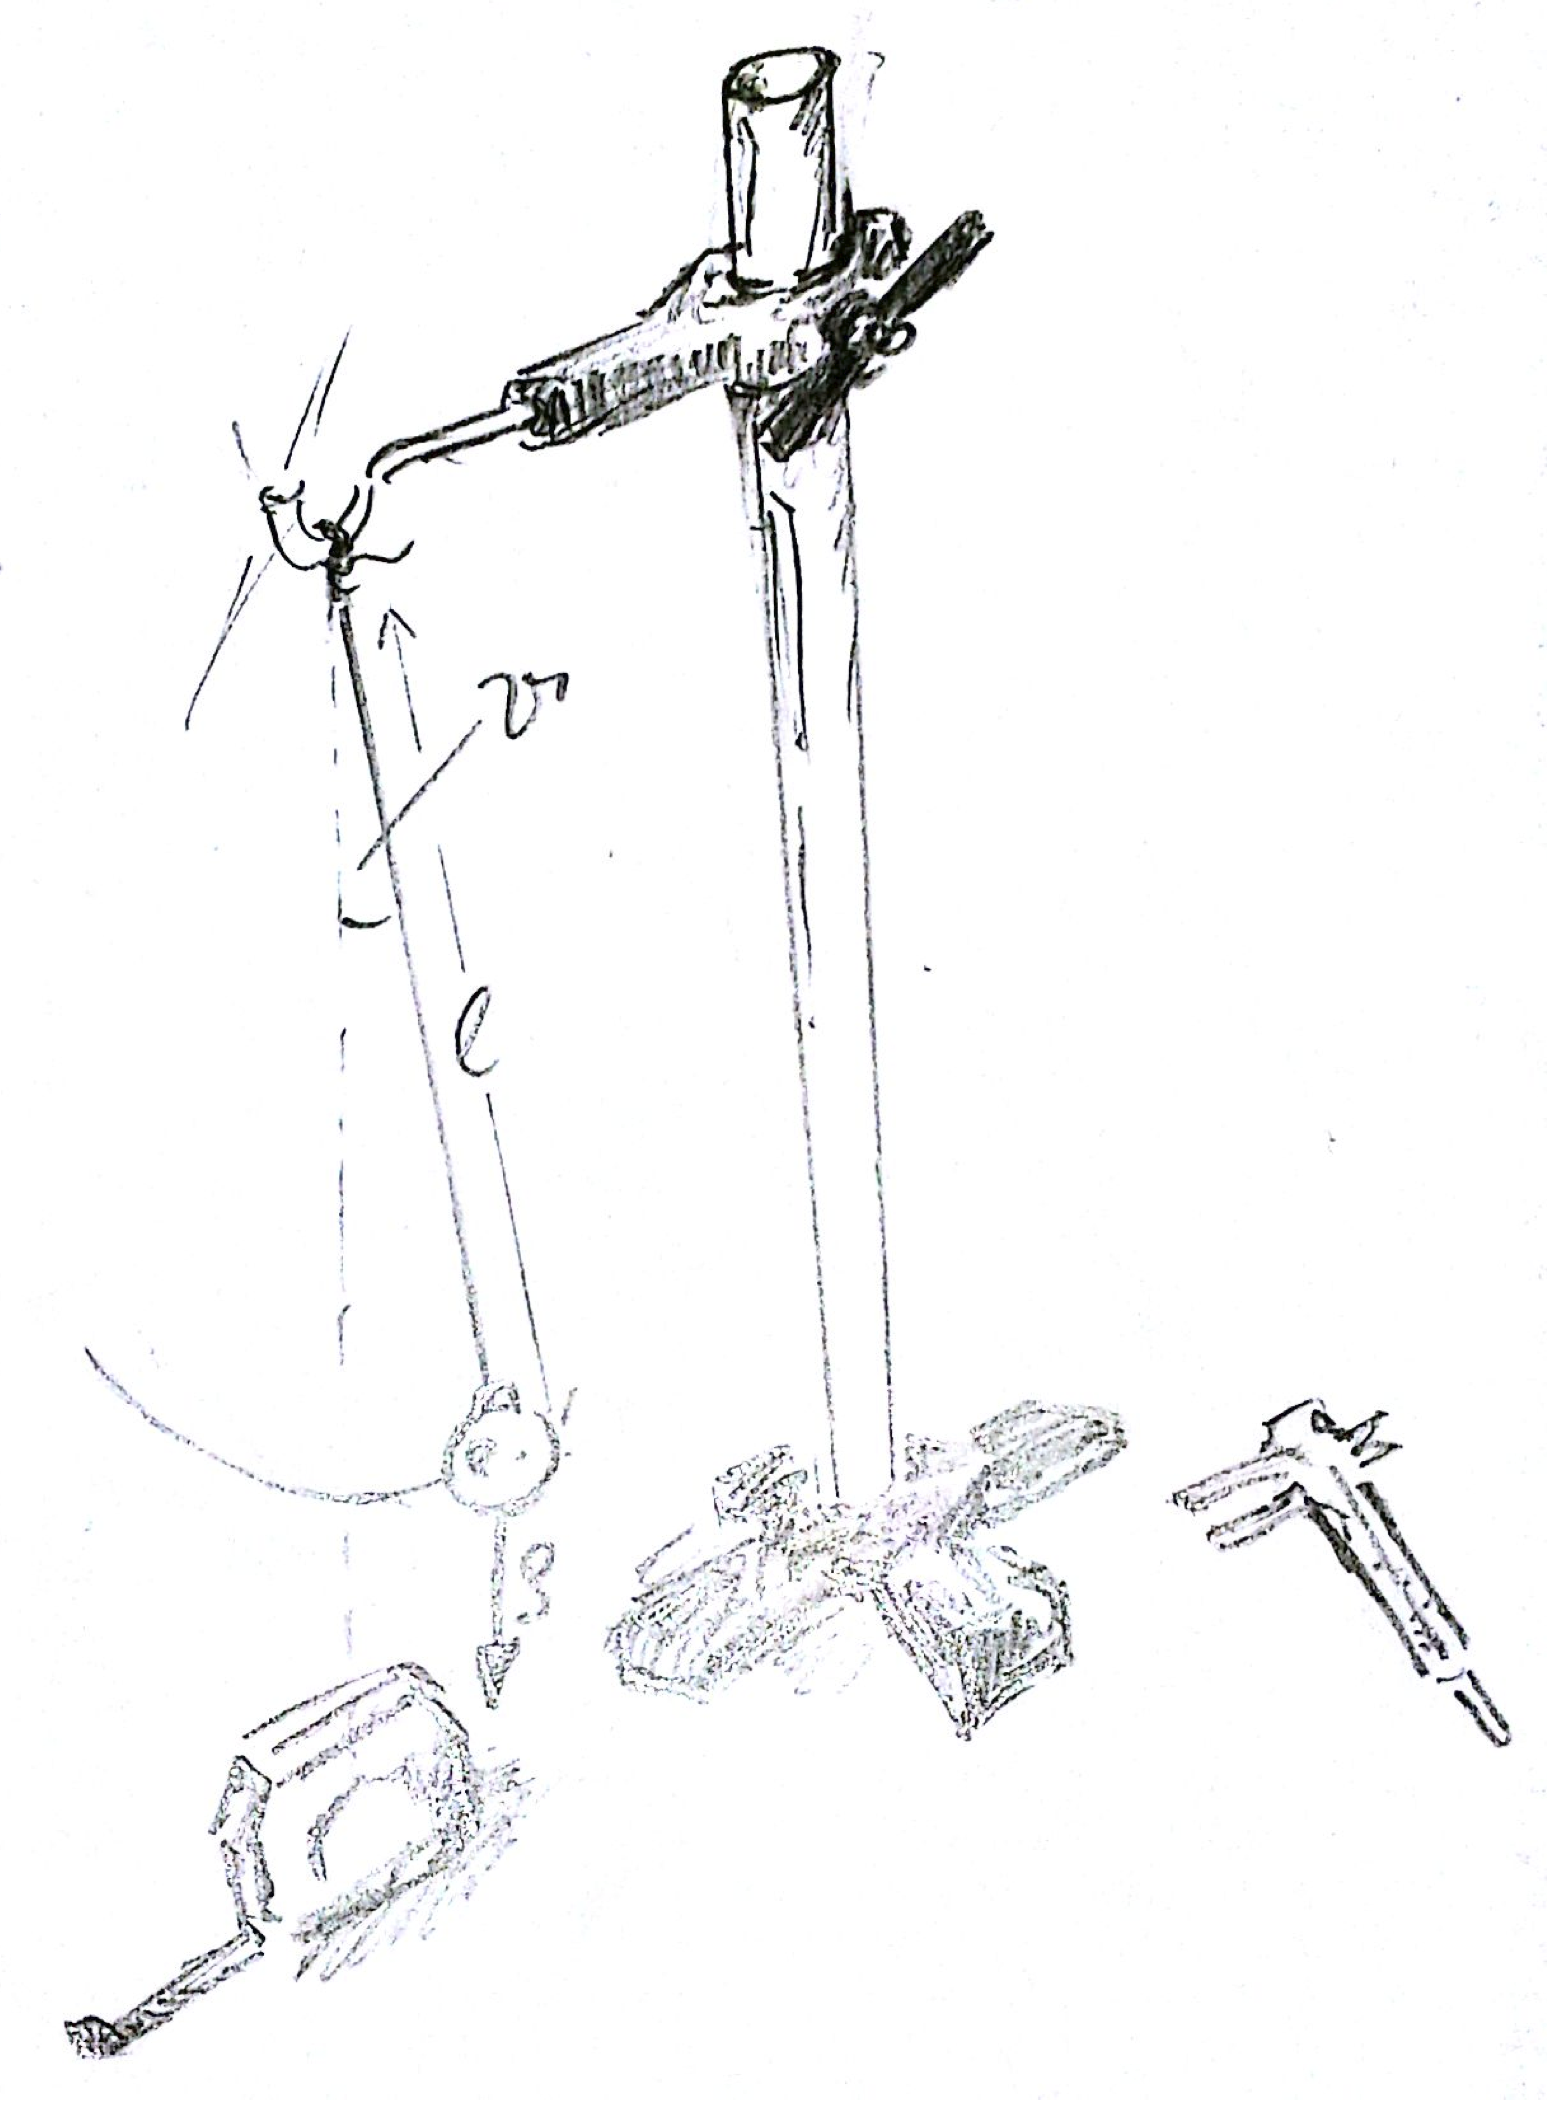
\includegraphics[scale=0.4]{./figure/pendel.png}
	\caption{Skizzierte Darstellung des Versuchsaubaus}
	\label{fig:301}
\end{figure}
%"Aufgabenstellung in einem Satz" - Wir bestimmen die lokale Erdbeschleunigung über den Zusammenhang zwischen Länge und Periodendauer eines Fadenpendels.\\

%Über 6.3 Grad entsteht ein Fehler der über der Messunsicherheit liegt. \\
%Messung bei Nulldurchgang.
%Messunsicherheit 1/100 Sekunden.
Durch ein Pendel (Metallkugel am dünnem Faden) wird ein mathematisches Pendel im Experiment angenähert. Da in diesem (theoretischen) System die Schwingungsdauer nur von der Länge des Pendels und der Erdbeschleunigung abhängt, soll im Experiment durch Messen der Schwingungsdauer sowie der Länge des Pendels, die Erdbeschleunigung berechnet werden.\\
\\
\\
\textbf{Equipment:}\\
\begin{itemize}
	\item Ein Pendel an einem Gestänge (schreibtischgroßer Aufbau)
	\item Ein Maßband (Auflösung 1mm)
	\item Eine Schieblehre (Auflösung 0.05mm)
	\item Eine Stoppuhr (Auflösung 0.01s)
\end{itemize}
Für kleine Winkel (und nach Umformung der Gleichung für die Schwingungsdauer nach der Erdbeschleunigung g), hängt g nur von der Länge l des Pendels sowie der Schwingungsdauer T im Quadrat ab.\\
Im ersten Schritt wird daher die Länge des Pendels gemessen. Da das verwendete Pendel, im Gegensatz zum idealisierten, keine unendlich kleine Punktmasse sondern eine Metallkugel ist, nehmen wir deren Schwerpunkt als den Ort der Masse. Es muss also die Fadenlänge mit dem Maßband, und der Durchmesser der Kugel mit der Schieblehre gemessen werden. Die Länge l ist schließlich Fadenlänge + halber Durchmesser der Kugel.\\
Danach wird die Schwingungsdauer des Pendels gemessen. Das wird in diesem Versuch einfach per Stoppuhr gemacht.\\
Einige Dinge sind dabei zu beachten: \\
Der beste Zeitpunkt um die Uhr zu starten und zu stoppen, ist, wenn das Pendel die höchste kinetische Energie hat, also bei genau senkrechtem Faden.\\
Außerdem ist zu beachten, dass die Amplitude nicht zu groß ist. Schließlich wird mit der Kleinwinkelnäherung der sinus-Funktion gerechnet.\\
Da diese Methode sehr ungenau ist, führen wir sowohl eine Messreihe (10 Messungen) durch, in der jeweils die Dauer 1 ganzen Schwingung gemessen wird, sowie eine Messreihe zu jeweils 10 Schwingungen. Der Fehler, der allein durch das ungenaue manuelle Drücken der Stoppuhr entsteht, und der einmalig pro Messung und additiv ist, wird so, wenn man das Ergebnis durch 10 teilt um auf eine Schwingungsdauer zu kommen, auch durch 10 geteilt.\\
Außerdem markieren wir, mit den eingeschränkten zur Verfügung stehenden Mitteln (hier mit dem Maßband) möglichst gut und nahe am Pendel den Punkt, an dem gemessen wird, um noch höhere Präzision zu erreichen.
\\
Mit den gewonnenen Daten kann anschließend die Erdbeschleunigung berechnet werden.\\
\begin{equation}
	g = \frac{4*\pi^2*l}{T^2}
\end{equation}
\\
Eine 2. Methode ist das Umformen der Gleichung in die Form einer Geradengleichung, wo g die Steigung einer Geraden
$T^2$, abhängig von l ist. Da andere Gruppen den gleichen Versuch mit Pendeln mit anderer Länge durchführen, kann man die Werte mehrerer Pendel gegeneinander auftragen und durch lineare Regression eine Gerade annähern, aus deren Steigung sich ebenso die Erdbeschleunigung g berechnen lässt.\\
\begin{equation}
	T^2= \frac{4*pi^2*l}{g}
\end{equation}

\subsection{Ergebnisse der Messungen}
\textbf{10 Einzelschwingungen}\\
Zur Berechnung des Fehlers haben wir die Gauss'sche Fehlerfortpflanzung verwendet.
Kugeldurchmesser: (1.995 $\pm 0.005$)cm\\
Seillänge: (62.1 $\pm  0.1$)cm\\
Bis Schwerpunkt: (63.0 $\pm$ 0.2)cm\\
Statistische Werte (QTIPlot):\\
Mittelwert: 1.58s, Standardabweichung: 0.0207s, Standard Fehler (u): 0.00657s, Varianz: 0.00043s\\
\pgfplotstabletypeset[fixed zerofill,precision=2]{
s 
1.59 
1.59 
1.63 
1.57 
1.58
1.57
1.56
1.59
1.56
1.57
}\\
\\
\textbf{10 Mehrfachschwingungen}\\
Statistische Werte (QTIPlot):\\
Mittelwert: 15.808s, Standardabweichung: 0.0031s, Standard Fehler (u): 0.000986s, Varianz : 9.73 $10^{-6}s$\\
\\
\pgfplotstabletypeset[fixed zerofill,precision=2]{
s 
15.91
15.91
15.89
15.92
15.94
15.83
15.93
15.90
15.92
15.93
}\\
Zusätzlich: 15.78s (Ausreisser, nicht mit einbezogen)\\
\subsection{Lineare Regression mit Gruppenergebnissen}

\begin{tikzpicture}
    \pgfplotsset{width=7cm,
        	compat=1.3,
        	legend style={font=\footnotesize}
	}
    \begin{axis}[
    xlabel={l[m]},
    ylabel={$T^2 [s^2]$ },
    legend cell align=left,
    legend style={at={(0.5,-0.3)},anchor=north}]
    \addplot[only marks] table[row sep=\\]{
        T l\\
        0.48 1.95\\
        0.63 2.53\\
        0.745 2.99\\
        0.276 1.12\\
    };
    \addlegendentry{Messpunkte}
    \addplot+[no markers] table[row sep=\\,
    y={create col/linear regression={y=l}}] % compute a linear regression from the
    %input table
    {
        T l\\
        0.48 1.95\\
        0.63 2.53\\
        0.745 2.99\\
        0.276 1.12\\
    };
    \addlegendentry{%
        $\pgfmathprintnumber{\pgfplotstableregressiona} \cdot x
        \pgfmathprintnumber[print sign]{\pgfplotstableregressionb}$ lin. Regression} %
    \end{axis}
    \end{tikzpicture}
\\
\\
$A = 3.9807 \pm 0.0255 \frac{m}{s^2} = \frac{4 \pi^2}{g}$\\
$\frac{\Delta A}{A} = \frac{\Delta g}{g}$\\
$\Delta g = 0.07 \frac{m}{s^2}$\\
$g = \frac{4 \pi^2}{3.9807 \pm 0.0255 \frac{m}{s^2}} = 9.92 \pm 0.07 \frac{m}{s^2}$\\

\subsection{Diskussion}
Angesichts der Messmethode, die zahlreiche Annäherungen beinhält (kein ideales math. Pendel, Kleinwinkelnäherung, menschlicher Messtrigger), ist, vor allem das Ergebnis aus der Messreihe mit 10 Schwingungen überraschend nahe am Literaturwert
$9.81 \frac{m}{s^2}\footnote{\url{http:\\de.wikipedia.org/wiki/Erdbeschleunigung}}$.
Der Vollständigkeit halber soll erwähnt sein, dass aus der Messreihe mit 10 Schwingungen 1 Wert entfernt wurde und durch eine neue Messung ersetzt, der mit 15.78s weit außerhalb der Streuung der anderen Werte lag, sowie schon beim zusehen und zuhören (Klick der Stoppuhr) unsauber wirkte.\\
Da die anderen Werte (ohne, dass zum Zeitpunkt der Messung schon das Ergebnis für g bekannt war, und damit ein Bias unsererseits ausgeschlossen war) um einen gemeinsamen Mittelwert streuen, halten wir dieses Vorgehen für eine unbedenkliche Korrektur einer Fehlmessung, und nicht für eine Ergebnisverzerrung.\\
Ein nahe liegender Schluss aus den Ergebnissen ist der, dass von den möglichen Fehlern und Unsicherheiten, die Messung durch menschliche Sinne den größten Effekt hat. Fehler, die durch Reibung, oder sonstige nicht-ideale Eigenschaften des Pendels entstehen, sollten sich bei mehreren Schwingungen eher vergrößern, dennoch ist diese Messung sehr viel genauer.\\
Dennoch liegt der Literaturwert zwar im Unsicherheitsbereich der 1-Schwingungs-Messung, nicht jedoch in dem der 10-Schwingungs-Messung, was an der weit größeren Unsicherheit der Einzelmessung liegt. Diese hat ihre Ursache wiederum in der viel größeren Streuung der Messwerte. \\
Es zeigt sich also, dass diese sehr einfache Methode, durchaus ein gutes Ergebnis liefern kann.\\
Die 2. Methode zur Berechnung der Erdbeschleunigung ergibt sich durch Umformung der Berechnungsformel in eine Geradengleichung $T^2(l)$ wobei g (mal einem Faktor $4*pi^2$) die Steigung ist.\\
Es soll erwähnt sein, dass die lineare Regression während dem Praktikumstermin gemeinsam mit 3 anderen Gruppen durchgeführt wurde. Durch ein technisches Problem steht uns diese Analyse nicht mehr zur Verfügung. Wir haben daher die Regression neu erstellt (siehe Abbildung \ref{fig:302}), verwenden jedoch hier die notierten Werte aus dem Gruppentermin (die jedoch erst in kleineren Größenordnungen als dem hier verwendeten Bereich für g von den hier dargestellten abweichen).\\
Die Steigung der Geraden steht in direktem linearen Zusammenhang mit g. Daher ist auch der Fehler direkt aus der Unsicherheit der Punkte im Bezug auf die Gerade gegeben.\\
Aus dieser Methode erhalten wir einen Wert von $g = (9.92 \pm 0.07) \frac{m}{s^2}$.\\
Verglichen mit dem Literaturwert ist dies doch deutlich ungenauer, als die beiden Messreihen. Da diese Methode eine Art von Mittelwert aller 4 Gruppen, die gleichzeitig dieses Experiment durchgeführt haben, zum Ergebnis hat, erzielt man damit nicht notwendigerweise höhere Genauigkeiten. Hier ist vor allem der lineare Zusammenhang interessant, die Messung lässt sich damit im Allgemeinen nicht unbedingt verbessern.\\
Abgesehen vom menschlichen Faktor, bringt möglicherweise die Länge des Pendels (größere Schwingungsdauer) genauere Ergebnisse, da der Nulldurchgang so einfacher abzuschätzen sein dürfte.
\section{Einfache elektrische Messungen}
In verschiedenen einfachen Schaltungen soll zunächst ein Ohmscher Widerstand, danach die Kapazität eines Kondensators gemessen werden. Der Widerstand wird sowohl mit einer Gleichstrom-Spannungsquelle, wie auch mit Wechselspannung gemessen, es kommen Serien- und Parallelschaltungen zum Einsatz.\\
Außerdem werden in den Aufgaben sowohl Spannungen als auch Ströme gemessen, wobei die Vor- und Nachteile des jeweiligen Betriebes des Multimeters, sowie deren Schaltung (spannungs- oder stromrichtig) auch ein Thema dieses Versuches sein sollen.\\
Um aus den gemessenen Werten den unbekannten Widerstand zu berechnen, benötigt man schließlich für die Gleichstromaufgaben die Kirchhoffschen Regeln sowie das Ohmsche Gesetz.\\
Um die Kapazität des Kondensators zu berechnen, ist es schließlich nötig, die österreichische Netzfrequenz, 50Hz, zu kennen.\\
\\
\textbf{Equipment:}\\
\begin{itemize}
	\item Zwei Fluke 175 True Multimeter 
	\item Ein Steckbrett
	\item Zwei Ohmsche Widerstände, einer davon unbekannt
	\item Ein Kondensator
	\item einige Kabel
\end{itemize}
\textbf{Betriebsarten der Multimeter:}\\
Gleichpannung:   Auflösung 10mV, Unsicherheit $\pm (0.15\% + 2)$\\
Wechselspannung: Auflösung 10mV, Unsicherheit $\pm (1\% + 3)$\\
Gleichstrom:     Auflösung 0.01 mA, Unsicherheit $\pm (1\% + 3)$\\
Wechselstrom:    Auflösung 0.01 mA, Unsicherheit $\pm (1\% + 3)$\\
\subsection{Aufgaben und Aufbau}
Der erste Teil des Versuchs, beschäftigt sich mit der Messung eines unbekannten Widerstandes $R_{x}$ auf verschiedene Arten bei Gleichstrom. Anhand der Ergebnisse lassen sich die verschiedenen Methoden vergleichen.\\
Zuerst wird der Widerstand sowohl in einer spannungs- als auch stromrichtigen Schaltung bestimmt (Abbildung \ref{fig:401}).\\
Danach wird er, in Parallelschaltung mit einem bekannten Widerstand R, durch Berechnung aus Gesamtstrom und -spannung ermittelt (Abbildung \ref{fig:402}).\\
Ebenso in Serienschaltung der beiden Widerstände (Abbildung \ref{fig:403}).\\
Zuletzt sollen, ebenso in Serie, die Spannungen an beiden Widerständen $R_{x}$ und R gemessen werden, und daraus $R_{x}$ berechnet werden (Abbildung \ref{fig:404}).\\
\\
Im zweiten Teil werden die Schaltungen mit Wechselstrom versorgt:\\
Einerseits wird wieder $R_{x}$ bestimmt, in Serienschaltung mit R, sowohl durch Messung von Gesamtstrom und -spannung, als auch durch Messung der Teilspannungen (Abbildung \ref{fig:405}).\\
Außerdem wird die Kapazität C eines Kondensators, und sein komplexer Wechselstromwiderstand $X_{c}$, bestimmt durch Messung der gleichen Größen (Also nochmalige Durchführung der Messung wie in Schaltung (Abbildung \ref{fig:405}) mit dem Kondensator statt $R_{x}$).\\
\\
Dabei ist vor allem auf die richtigen Einstellungen an den Multimetern zu achten, je nach zu messender Größe und verwendetem Strom. Außerdem lässt sich der Versuch durch strategisch günstiges Stecken der einzelnen Schaltungen wesentlich beschleunigen und die Fehleranfälligkeit durch klare aufgeräumte Schaltungen verringern.\\
\\
\\

\subsection{Ergebnisse der Messungen}
\textbf{$R_{x}$ stromrichtig:}\\
$I = (8.89 \pm 0.12) mA$\\
$U = (24.01 \pm 0.06) V$ \\
$R_{x} = \frac{U}{I} = (2.701 \pm 0.002) k\Omega$\\
\\
\textbf{$R_{x}$ spannungsrichtig:}\\
$I = (8.90 \pm 0.12) mA$\\
$U = (24.00 \pm 0.06) V$ \\
$R_{x} = (2.697 \pm 0.003) k\Omega$\\
\\
\textbf{Parallelschaltung mit R (4.7k$\Omega$)}\\
$I_{ges} = (14.03 \pm 0.17) mA$\\
$U_{ges} = (23.98 \pm 0.06) V$\\
$R_{x} = \frac{U_{ges} - \frac{1}{R} }{ I_{ges} } = (2.686 \pm 0.028) k\Omega$ \\
\\
\textbf{Serienschaltung mit (4.7k$\Omega$)}\\
$I_{ges} = (3.25 \pm 0.07) mA$\\
$U_{ges} = (24.01 \pm 0.06) V$\\
$R_{x} = R_{ges} - R = (2.688 \pm 0.058) k\Omega$\\
\\
\textbf{Serienschaltung, 2 Teilspannungen}\\
$U_{R} = (15.22 \pm 0.05) V$\\
$U_{R_{x}} = (8.80 \pm 0.04) V$\\
$R_{x} = \frac{R*U_{R_{x}}}{U_{R}} = (2.717 \pm 0.016) k\Omega$\\
\\
\textbf{Serienschaltung, Wechselstrom, Gesamtstrom und -Spannung}\\
$I_{ges} = (3.69 \pm 0.07) mA$\\
$U_{ges} = (27.08 \pm 0.30) V$\\
$R_{x} = R_{ges} - R = (2.639 \pm 0.058) k\Omega$\\
\\
\textbf{Serienschaltung, Wechselstrom, 2 Teilspannungen}\\
$U_{R} = (17.19 \pm 0.21) V$\\
$U_{R_{x}} = (9.93 \pm 0.13) V$\\
$R_{x} = \frac{R*U_{R_{x}}}{U_{R}} = (2.715 \pm 0.049) k\Omega$\\
\\
\textbf{Serienschaltung, Kondensator}\\
$I_{ges} = (3.19 \pm 0.07) mA$\\
$U_{ges} = (27.15 \pm 0.30) V$\\
$U_{R} = (14.83 \pm 0.18) V$\\
$U_{C} = (22.65 \pm 0.26) V$\\
$\omega = 2*\pi *50$ \\
$X_{c} = \frac{U_{C}}{I_{ges} - R} = (3.811 \pm 0.094) k\Omega$ \\
$C = (\omega * X_{c})^{-1} = 835 \pm 21 nF$ \\

\end{multicols}
\section{Quellen}
Formeln und Abbildungen für Schaltungen aus Anleitung PW1 \url{http://www.univie.ac.at/anfpra/neu1/pw/pw1/PW1.pdf} und dem Leitfaden \url{http://www.univie.ac.at/anfpra/neu1/organisation/ablaufDurchfuehrung/leitfaden.pdf}.
\end{document}